\documentclass{article}

\usepackage{booktabs} 
\usepackage[english]{babel}
\usepackage{graphicx}
\usepackage{amsmath}
\usepackage{wrapfig}

\title {Written Assignment 3}
\date{6 November 2016}
\author{Wendy Nieuwkamer}

\begin{document}

\maketitle

\section{Question 3}
\textit{We have a Neural Network with 1 hidden layer. Input and hidden layer both have 2 nodes. There is 1 output node. the values of theta for bias nodes are 0.2.
The vector $\theta^{(1)}$ for layer 1 is: [0.5,0.1,0.5,0.7] and $\theta^{(2)}$ for layer 2 is [1,2].}

This information can be visualized in a directed graph like I did in figure 1.

\begin{figure} [h!]
	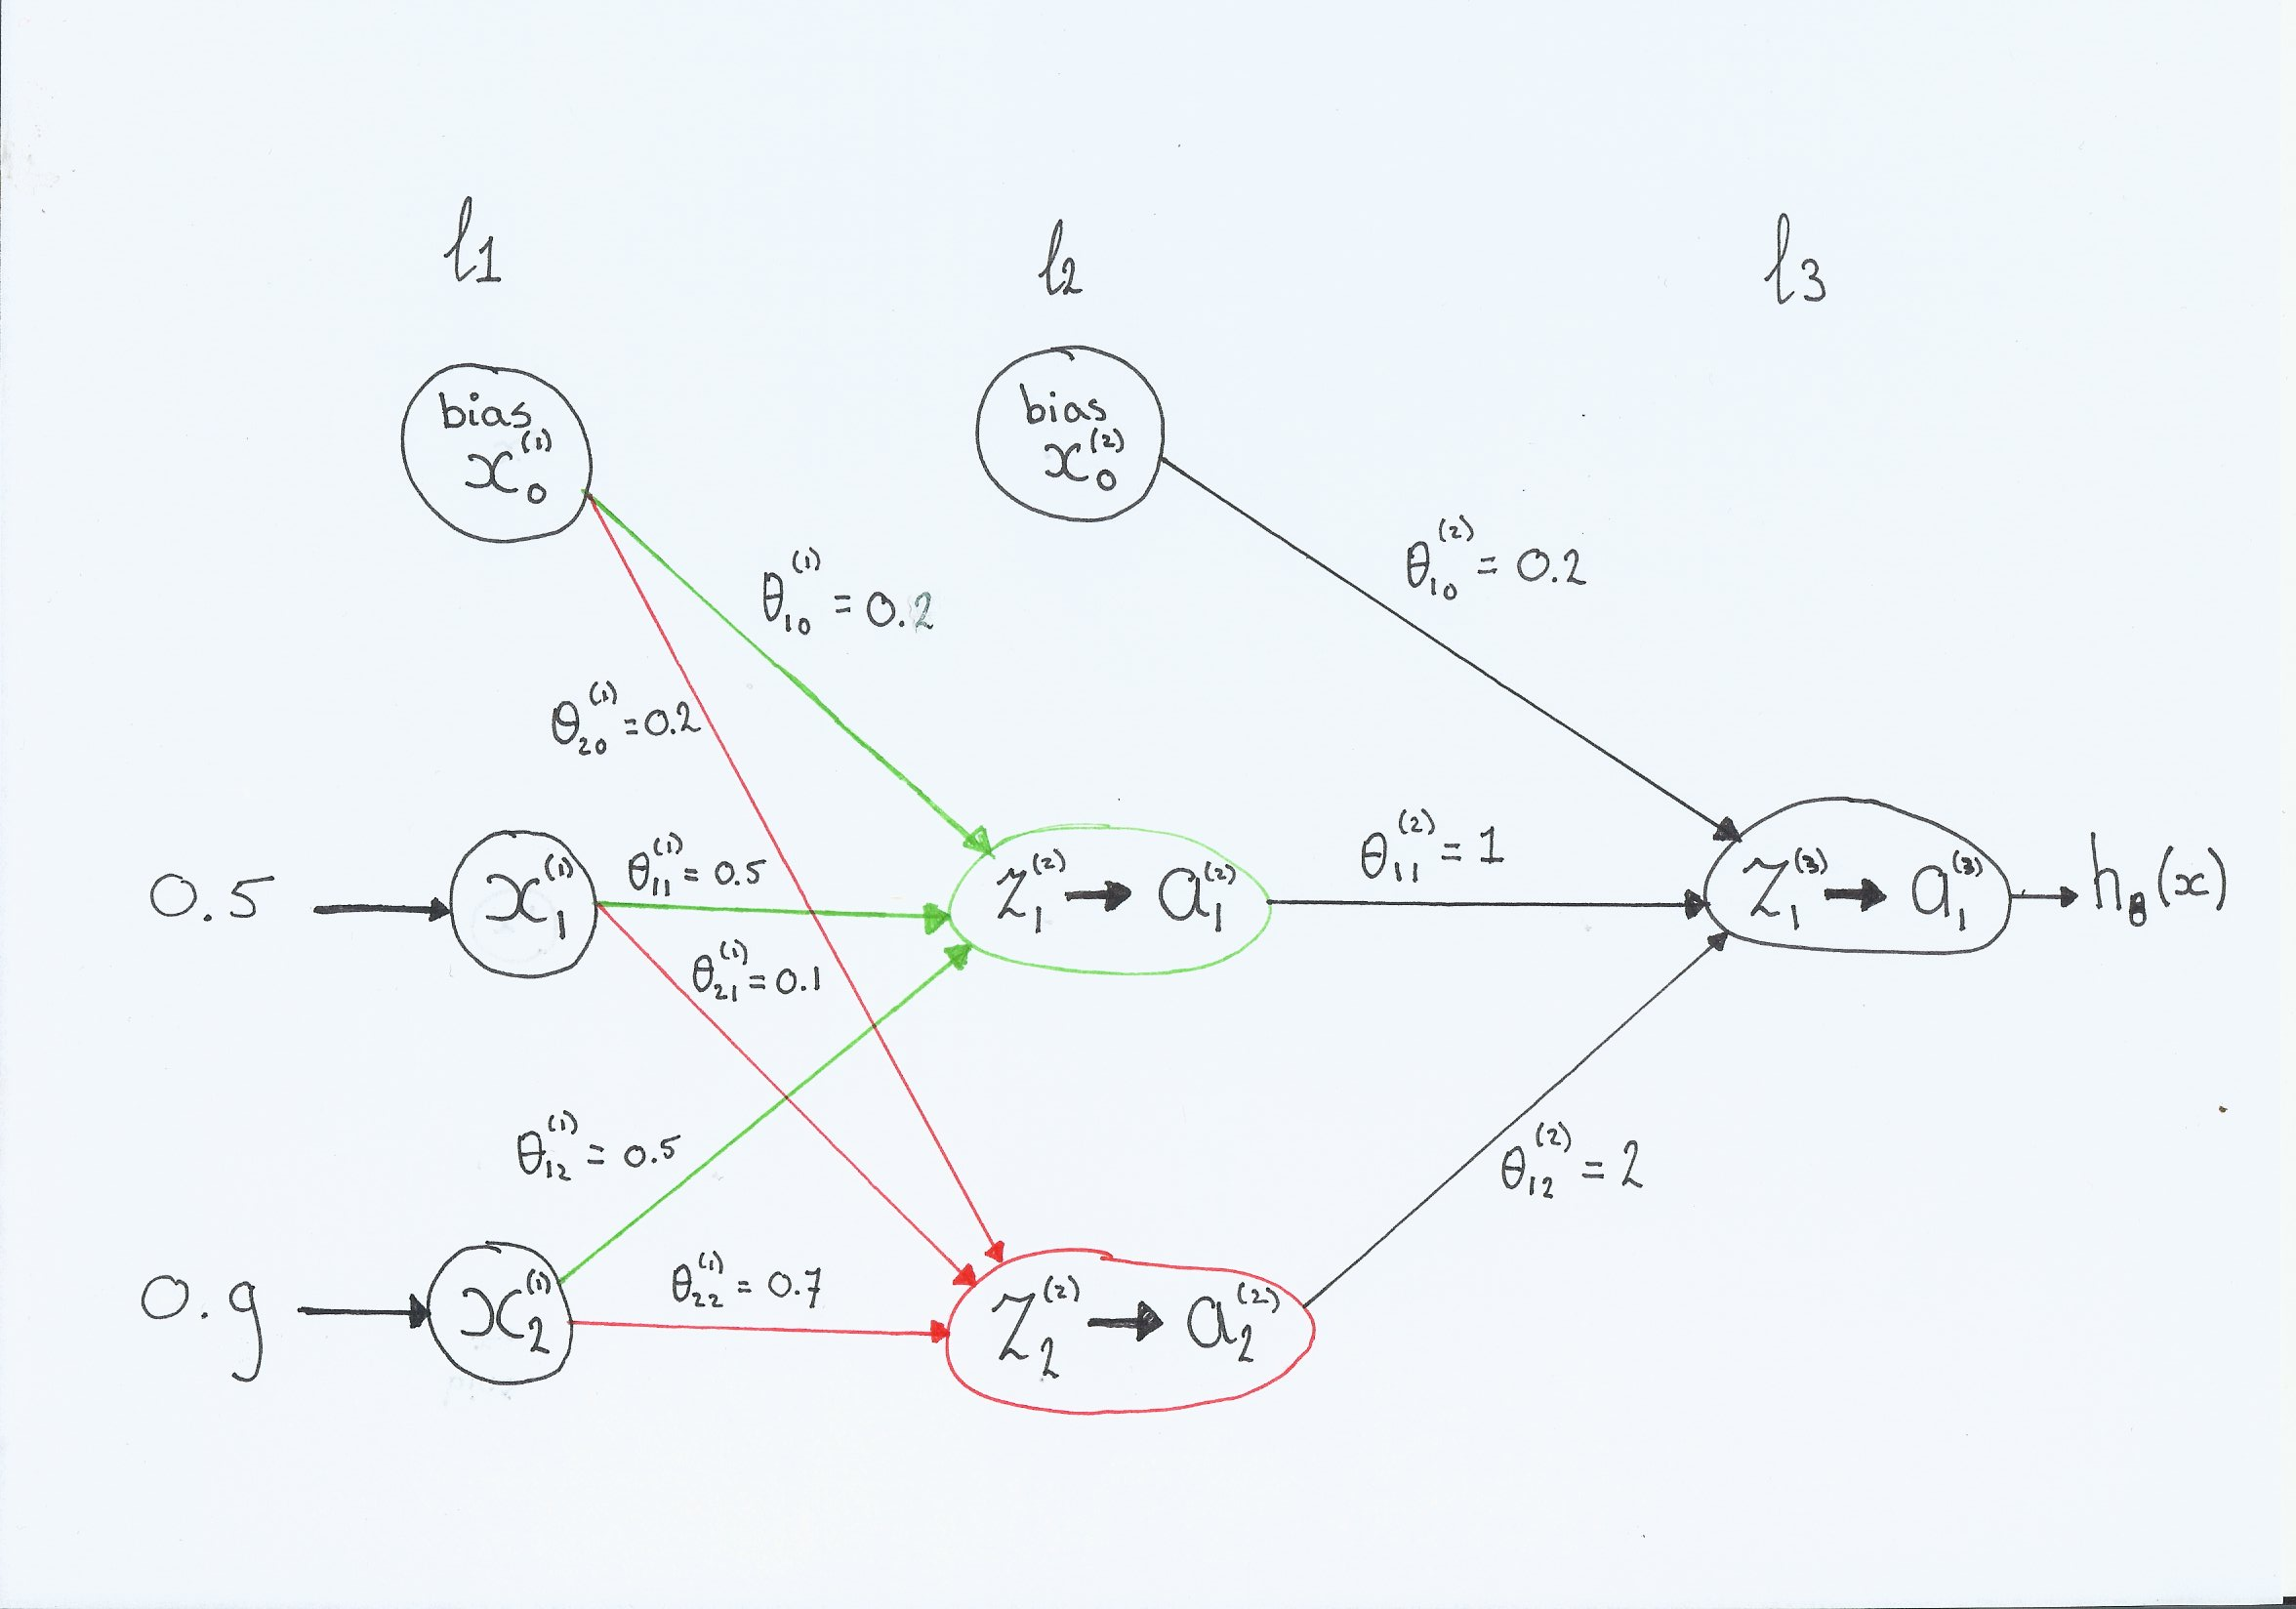
\includegraphics[width=\linewidth]{NeuralNetwork.JPG}
	\caption{Our Neural Network}
	\label{fig:network}
\end{figure}

\subsection{Calculate by hand the activations of all nodes for $x_1 = 0.5$ and $x_2 = 0.9$. }

We go layer by layer. For each node in a layer we first calculate the $z$ value. We do this by taking the sum of all the inputs multiplied by their weights. 
\begin{align*}
z^{(2)}_1 &= \theta_{10}^{(1)}x_0^{(1)} +  \theta_{11}^{(1)}x_1^{(1)} +  \theta_{12}^{(1)}x_2^{(1)} \\
&= 0.2 \cdot 1 + 0.5 \cdot 0.5 + 0.5 \cdot 0.9 \\
&= 0.2 + 0.25 + 0.45 \\
&= 0.9 \\
 \\
z^{(2)}_2 &= \theta_{20}^{(1)}x_0^{(1)} +  \theta_{11}^{(1)}x_1^{(1)} +  \theta_{12}^{(1)}x_2^{(1)} \\
&=0.2 \cdot 1 + 0.1 \cdot 0.5 + 0.7 \cdot 0.9 \\
&= 0.2 + 0.05 + 0.63 \\
&= 0.88
\end{align*}

The we calculate the activation value for each node using the sigmoid function:
\begin{equation*}
g(z) = \frac{1}{1 + e^{-z}}
\end{equation*}

\begin{align*}
a^{(2)}_1 &= \frac{1}{1 + e^{-z^{(2)}_1}} \\
&=  \frac{1}{1 + e^{-0.9}} \\
&= 0.7109 \\
\\
a^{(2)}_2 &= \frac{1}{1 + e^{-z^{(2)}_2}} \\
&=  \frac{1}{1 + e^{-0.88}} \\
&= 0.7068
\end{align*}

\pagebreak

The third and last layer will then be:

\begin{align*}
z^{(3)}_1 &= \theta_{10}^{(2)}x_0^{(2)} +  \theta_{11}^{(2)}x_1^{(2)} +  \theta_{12}^{(2)}x_2^{(2)} \\
&=0.2 \cdot 1 + 1 \cdot 0.7109 + 2 \cdot 0.7068 \\
&= 0.2 + 0.7109 + 1.4136 \\
&= 2.3245 \\
\\
a^{(3)}_1 &= \frac{1}{1 + e^{-z^{(3)}_1}} \\
&=  \frac{1}{1 + e^{-2.3245}} \\
&= 0.9109
\end{align*}

Our final activation value is the hypothesis. Thus, in this case  $a^{(3)}_1  = h_\theta(x) = 0.9109$. 

\subsection{Suppose the correct output is 1. Calculate the errors for all nodes and the updates of the
weights (for 1 iteration).}
We will now execute a back propagation in order to calculate the $\delta$-values and update the weights ($\theta$) of our edges. 
$\delta_j^{(l)}$ is the "error" for a node $n_j^{(l)}$ in a network. It is calculated with the following equation:

\begin{equation*}
\delta_j^{(l)}  = \theta^{(l)} \delta^{(l+1)}
\end{equation*}

For the last node in the network we use a slightly different formula, namely, $\delta_j^{(l)} = y - a_j^{(l)} = h_\theta(x) - a_j^{(l)}$. In this case the last node in the network is $n_1^{(3)}$. After calculating this delta, we move one layer back and calculate the delta values. We don't consider the first layer as these are our input values. 

\begin{align*}
\delta_1^{(3)} &= y - a_1^{(3)} \\
&= 1 - 0.9109 \\
&= 0.0891 \\
\\
\delta_1^{(2)} &= \theta^{(2)}_{11}\delta_1^{(3)}\cdot g'(z_1^{(2)})\\
&=  \theta^{(2)}_{11}\delta_1^{(3)} \cdot a_1^{(2)}(1- a_1^{(2)})\\
&= 1 \cdot 0.0891 \cdot 0.7109 (1 - 0.7109) \\
&= 0.0183 \\
\\
\delta_2^{(2)} &= \theta_{12}^{(2)} \delta_1^{(3)} \cdot a_2^{(2)}(1-a_2^{(2)}) \\
&= 2 \cdot 0.0891 \cdot 0.7068 ( 1 - 0.7068) \\
&= 0.0369
\end{align*}

Now we have calculated the delta values we can use them to update the weights of the edges, in this case the theta values, using the following formula:

\begin{equation*}
\theta_{ij}^{(l)} := \theta_{ij}^{(l)} - \alpha a_j^{(l)} \delta_i^{(l+1)}
\end{equation*}
 
Choose the learning rate $\alpha = 1$ for convenience. We don't update the bias thetas as these are constant. If we would update them the purpose of them would be countered. Again we do this layer by layer. \\

Layer 1: 
\begin{align*}
\theta_{11}^{(2)} &:= \theta_{11}^{(2)} - \alpha a_1^{(2)} \delta_1^{(3)} \\
&= 1 -  1 \cdot 0.7109 \cdot 0.0891 \\
&= 0.9367 \\
\\
\theta_{12}^{(2)} &:= \theta_{12}^{(2)} - \alpha a_2^{(2)} \delta_1^{(3)}  \\
&= 2 - 1 \cdot 0.7068 \cdot 0.0891 \\
&= 1.9370
\end{align*}

Layer 2:
\begin{align*}
\theta_{11}^{(1)} &:= \theta_{11}^{(1)} - \alpha x_1^{(1)} \delta_1^{(2)} \\
&= 0.5 - 1 \cdot 0.5 \cdot 0.0183\\
&= 0.4909\\
\\
\theta_{12}^{(1)} &:= \theta_{12}^{(1)} - \alpha x_2^{(1)} \delta_1^{(2)} \\
&= 0.5 - 1 \cdot 0.9 \cdot 0.0183\\
&= 0.4835 \\
\\
\theta_{21}^{(1)} &:= \theta_{21}^{(1)} - \alpha x_1^{(1)} \delta_2^{(2)} \\
&= 0.1 - 1 \cdot  0.5 \cdot 0.0369 \\
&= 0.0816 \\
\\
\theta_{22}^{(1)} &:= \theta_{22}^{(1)} - \alpha x_2^{(1)} \delta_2^{(2)} \\
&= 0.7 - 1 \cdot 0.9 \cdot 0.0369\\
&= 0.6668
\end{align*}

In linear regression we use a similar process for every training example.

\pagebreak

\section{Question 4}
\textit{In this exercise you will use a perceptron (instead of sigmoid function), that is explained in the
slides of Mitchell. }
 
The perceptron is defined as follows:

\begin{figure} [h!]
	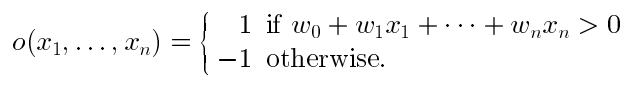
\includegraphics[width=\linewidth]{perceptronDef.png}
\end{figure}

\subsection{What are the values of weights $w_0$, $w_1$ and $w_2$ for the perceptron whose decision surface is
illustrated in figure \ref{fig:perc}}

\begin{wrapfigure} []{R}{0.25\textwidth}
\begin{center}
	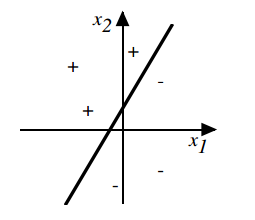
\includegraphics[width=100pt]{perceptron1.png}
\end{center}
	\caption{Decision Surface of a Perceptron}
	\label{fig:perc}
\end{wrapfigure}

\textit{Assume the surface crosses the $x_1$ axis at -1 and the $x_2$ axis at 2.}

Let's first write down the function of $x_2$ relative to $x_1$. Then we can rewrite it as a sum of x values which is equal to 0.

\begin{align*}
x_2 &= 2x_1 + 2\\
0&=2+2x_1-x_2
\end{align*}

As we can see in figure \ref{fig:perc}, all values under this surface should be 0 and everything above it should be 1. Thus, our weights will be $w_0 = 2$, $w_1 = 2$ and $w_2 = -1$.

\subsection{Designing perceptrons}
\subsubsection{Design a two-input perceptron that implements the Boolean function A AND (NOT B).}

Let's start with writing out the truth table for A AND (NOT B).

\begin{table}[h!]
\centering
\begin{tabular}{c c c c}
 A & B & NOT B & A AND (NOT B)\\
\hline
1&1&0&0\\
1&0&1&1\\
0&1&0&0\\
0&0&1&0
\end{tabular}
\end{table}

We have two input values, thus we need three weight values: \textit{Return 1 if $w_0 + w_1A + w_2 B > 0$, otherwise return 0}. A quick sketch gives us the possible values $w_0 = -0.5$, $w_1 = 1$ and $w_2 = -1$. Calculating the values for the summation and the corresponding gives us the following table:

\begin{table}[h!]
\centering
\begin{tabular}{c c c c}
 A & B & Sum & Output\\
\hline
1&1&-0.5&0\\
1&0&0.5&1\\
0&1&-1.5&0\\
0&0&-0.5&0
\end{tabular}
\end{table}

The outputs in this table is are the same as those in the truth table, thus we have found a perceptron for the boolean function A AND (NOT B). 

\subsubsection{Design a two-layer network of perceptrons that that implements A XOR B.}
Again, we start with writing out the truth table and a visualization on paper.

\begin{table}[h!]
\centering
\begin{tabular}{c c c }
 A & B & A XOR B\\
\hline
1&1&0\\
1&0&1\\
0&1&1\\
0&0&0
\end{tabular}
\end{table}

As this is not solvable with one perceptron we need a network. A XOR B is equivalent to $\lnot(A \land B) \land (A \lor B)$. Thus, in the first layer we can have the perceptrons for $ \not(A\land B)$ and $A\lor B$ and then feed the results to a AND perceptron in the second layer.\\

 $ \not(A\land B)$ with weights $w_0 = 1.5$, $w_1 = -1$ and $w_2 = -1$ gives the following outputs:

\begin{table}[h!]
\centering
\begin{tabular}{c c c }
 A & B & $ \not(A\land B)$\\
\hline
1&1&0\\
1&0&1\\
0&1&1\\
0&0&1
\end{tabular}
\end{table}

A OR B with the weights  $w_0 = -0.5$, $w_1 = 1$ and $w_2 = 1$ gives the following outputs:

\begin{table}[h!]
\centering
\begin{tabular}{c c c }
 A & B & $ A\lor B$\\
\hline
1&1&1\\
1&0&1\\
0&1&1\\
0&0&0
\end{tabular}
\end{table}

\pagebreak

Finally, feeding these inputs to the AND perceptron with weights $w_0 = 0.5$, $w_1 = -1$ and $w_2 = -1$ gives us the following outputs:

\begin{table}[h!]
\centering
\begin{tabular}{c c c c c}
 A & B & $ \not(A\land B)$& $ A \lor B$ & A XOR B\\
\hline
1&1&0 &1&0\\
1&0&1&1&1\\
0&1&1&1&1\\
0&0&1&0&0
\end{tabular}
\end{table}

This shows that our model is correct. 






\end{document}